\documentclass[conference]{IEEEtran}

\usepackage{cite}
\usepackage{amsmath,amssymb,amsfonts}
\usepackage{algorithmic}
\usepackage{graphicx}
\usepackage{textcomp}
\usepackage{xcolor}
\usepackage{booktabs}
\usepackage{placeins}
\usepackage{url}
\usepackage{array}
\usepackage{comment}

% Custom commands for consistency
\newcommand{\R}{\mathbb{R}}

\begin{document}

\title{AI-Integrated Edge-Fog IoT Architectures:\\ A PRISMA-Based Taxonomy and Systematic Review}

\author{\IEEEauthorblockN{Abeer Morgan}
\IEEEauthorblockA{\textit{Department of Information Technology} \\
\textit{Faculty of Computer and Information Technology} \\
\textit{Sana'a University}, Sana'a, Yemen \\
Email: abeer.murgan@su.edu.ye}
\and
\IEEEauthorblockN{Ahmed A. Shalabi}
\IEEEauthorblockA{\textit{Department of Information Technology} \\
\textit{Faculty of Computer and Information Technology} \\
\textit{University of Science and Technology}, Sana'a, Yemen \\
Email: a.alshalabi@su.edu.ye}
}

\maketitle

\begin{abstract}
The recent explosion of distributed Internet of Things (IoT) applications calls for adopting Edge-Fog computing as a necessary paradigm to tackle issues such as latency, scalability and WAN bandwidth constraints. Yet, current literature is somewhat fragmented as it focuses primarily on orchestration techniques separately from system design issues. In this study, we present a systematic literature review and three-dimensional taxonomy of artificial intelligence (AI) incorporation in Edge-Fog IoT systems, which follow PRISMA guidelines. The results of our analysis of 30 peer-reviewed papers, released between 2020 and 2025 in IEEE Xplore, ScienceDirect, MDPI and Google Scholar, provide categorization of state-of-the-art systems on three key dimensions: architectural configuration (layered and hybrid approach); intelligence nature (machine learning, deep learning and reinforcement learning); and functionality type (offloading tasks and managing resources). Our analysis reveals key technical compromises made in such systems; namely, the fact that reinforcement and deep learning approaches increase the system flexibility in exchange for heavy computation and convergence overhead, which makes them difficult to deploy at resource-constrained edges. We also explore security-computation and simulation-reality gaps of the studied literature. Finally, based on our findings, we discuss a research agenda for further work, including development of light-weight edge intelligence techniques, energy-aware orchestration algorithms and extensive real-world experimentation.

\end{abstract}

\begin{IEEEkeywords}
Edge Computing, Fog Computing, Internet of Things (IoT), Artificial Intelligence, Systematic Review, PRISMA, Resource Management, Task Offloading, Taxonomy.
\end{IEEEkeywords}

\section{Introduction}
\label{sec:intro}

The rise of the IoT ecosystem networking raises the need to create extremely distributed and data-driven architectures capable of performing real-time processing with ultra-low latencies. As the traditional cloud-based architecture cannot solve this challenge due to the presence of communication latency and high WAN transmission costs \cite{b1,b5}, the introduction of Edge/Fog computing has become inevitable for the reduction of network latency and real-time processing in a decentralized system \cite{b22,b23}.

Still, the deployment of scalable Edge/Fog architectures encounters the challenge related to the nature of edge devices themselves. Specifically, edge devices are characterized by limited computation and power supply capacity and limited storage resources while the cloud is still the only tier for processing intensive tasks; however, it is too distant and creates high latencies \cite{b6,b20}. This challenge acquires great significance for time-critical IoT applications with changing workload and diverse devices \cite{b21}. In this respect, nowadays researchers pay particular attention to incorporating Artificial Intelligence (AI) into IoT systems \cite{b4,b9}.


\subsection{Research Gaps and Motivation}
However, despite the fast-growing research in the area of interaction between AI and Edge-Fog Computing, literature is still very heterogeneous. Even though several surveys of the IoT architecture and intelligent computing paradigm exist \cite{b10,b15}, the analysis is made separately from each other. For example, researchers consider separate algorithms of task offloading \cite{b3} or energy efficiency \cite{b7} without considering the IoT architecture as a co-designed and integrated resource and network one.

Moreover, no systematic survey paper provides a systematic protocol of selection criteria, thus creating a selection bias. The majority of papers do not contain a quality assessment criterion, which makes it hard to verify the empirical validity of the solution provided by the author. Thus, the purpose of this work is to conduct a systematic survey based on the PRISMA protocol \cite{b31}.


\subsection{Positioning Against Existing Surveys}
To clarify the novel contributions of this study, Table~\ref{tab:survey_comparison} compares this work with representative surveys in the Edge-Fog IoT domain.


\begin{table*}[t]
\centering
\caption{Technical Comparison of the Proposed Review Against Existing Surveys}
\label{tab:survey_comparison}

\small
\setlength{\tabcolsep}{5pt}
\renewcommand{\arraystretch}{1.15}

\begin{tabular}{lccccccp{5.7cm}}
\toprule
\textbf{Reference} &
\textbf{Year} &
\textbf{Studies} &
\textbf{PRISMA} &
\textbf{Arch.} &
\textbf{AI} &
\textbf{Func.} &
\textbf{Main Contribution} \\
\midrule

Chang et al. \cite{b1}
& 2021
& -- 
& No
& Low
& High
& Med.
& General principles and trends in AI-enabled IoT systems. \\

Sheikh et al. \cite{b5}
& 2025
& --
& No
& Med.
& Low
& Low
& Classification of security threats and mitigation strategies. \\

Khan et al. \cite{b9}
& 2025
& 78
& Yes
& Med.
& Med.
& High
& Systematic coverage of ML-based resource management in fog computing. \\

Hosseinzadeh et al. \cite{b10}
& 2023
& 65
& Yes
& Med.
& Low
& High
& Classification of task-scheduling mechanisms in fog environments. \\

Costa et al. \cite{b15}
& 2022
& --
& No
& High
& Low
& High
& Broad survey of fog orchestration mechanisms and platforms. \\

Vali et al. \cite{b24}
& 2026
& --
& No
& High
& Low
& High
& Review of microservices-based resource management in fog and edge systems. \\

Cajas et al. \cite{b28}
& 2025
& --
& No
& Med.
& High
& Med.
& Survey of intelligent edge computing and ML optimization techniques. \\

\textbf{This Work}
& \textbf{2026}
& \textbf{30}
& \textbf{Yes}
& \textbf{3-Tier}
& \textbf{ML/DL/RL}
& \textbf{Joint}
& \textbf{PRISMA-based three-dimensional taxonomy integrating architecture, intelligence, and functionality.} \\

\bottomrule
\end{tabular}
\end{table*}


Table~\ref{tab:survey_comparison} clearly highlights the fact that current surveys mainly emphasize the isolated dimensions like security, orchestration, scheduling of tasks or machine learning-enabled resource management. Not only that but some surveys do not follow the PRISMA framework approach which further diminishes the credibility of the selection process of the surveys. This study on the other hand is a systematic, quality assessed survey in which the architectural design, intelligence and functionality of the system have been considered in a three dimensional way.


\subsection{Summary of Contributions}
The core contributions of this systematic review are:
\begin{itemize}
    \item \textbf{A Methodologically Rigorous Literature Mapping:} We use the PRISMA 2020 checklist for screening a total of 110 articles and select 30 good-quality articles between the years 2020
    \item \textbf{A Novel Three-Dimensional Taxonomy:} Literature is classified into categories by means of Architecture Type (Layered or Hybrid), Intelligence Type (ML, DL, RL, Hybrid), and System Functionality (Offloading or Resource Management).

    \item \textbf{Critical Synthesis of Technical Impasses:} We examine the following system bottlenecks in detail: computation-latency conflicts, security-computation conflict, and the reality-simulation deployment challenge.
    \item \textbf{Strategic Research Roadmap:} These directions include lightweight intelligence, energy-efficient orchestration, and validation through physical testbeds.
\end{itemize}


The rest of this paper is structured as follows. Section~\ref{sec:methodology} describes the systematic approach for literature search and selection criteria. Section~\ref{sec:taxonomy} introduces the proposed three-dimensional taxonomy. Section~\ref{sec:mapping} describes the study mapping and quality assessment matrix. Section~\ref{sec:quantitative} describes the quantiative study analysis. Section~\ref{sec:impasses} analyzes the critical technical impasses. Section~\ref{sec:trends} introduces the trends and future roadmaps.


\section{Research Methodology (PRISMA-Based)}
\label{sec:methodology}

To ensure reproducibility, transparency, and scientific rigor, we employed the Preferred Reporting Items for Systematic Reviews and Meta-Analyses (PRISMA) 2020 guidelines \cite{b31}.

\subsection{Search Strategy and Data Sources}
A systematic search was carried out in four prominent academic databases: IEEE Xplore, Elsevier’s ScienceDirect, MDPI, and Google Scholar. The Boolean search query for the literature review was formulated based on terms associated with architecture, intelligence, and functionalities of Edge-Fog IoT environments. The search query is given below:

\begin{quotation}
\texttt{("Edge-Fog" OR "Fog Computing" OR "Edge-Fog IoT") AND ("Artificial Intelligence" OR "Machine Learning" OR "Deep Learning" OR "Reinforcement Learning") AND ("Resource Management" OR "Task Offloading" OR "Orchestration")}
\end{quotation}

To capture the state-of-the-art developments, searches were restricted to articles published between \textbf{2020 and 2025}. Google Scholar was treated as a supplementary database to cross-check for gray literature, where the first 50 results were systematically screened based on relevance.

\subsection{Selection Criteria and Exclusion Decisions}
We applied a strict selection workflow. To maintain a high quality threshold, we restricted our core scope to peer-reviewed journal articles, excluding conference articles and preprints. While we acknowledge that conferences are primary venues for emerging IoT protocols, peer-reviewed journals offer complete details on mathematical modeling and empirical validation. To avoid excluding critical advancements, we included journals that expand upon prior conference papers.

The screening process operated as follows:
\begin{enumerate}
    \item \textbf{Inclusion Criteria:} (a) Must propose an architecture spanning both the edge and fog tiers (and optionally cloud); (b) Must utilize an AI, ML, DL, or RL model for optimization; (c) Must evaluate performance using quantitative metrics (latency, energy, cost, accuracy).
    \item \textbf{Exclusion Criteria:} (a) Papers focusing on cloud-edge scheduling without intermediate fog gateways; (b) Purely descriptive or narrative studies without mathematical models; (c) Non-peer-reviewed papers.
\end{enumerate}

From the initial pool of 110 retrieved documents, 15 duplicates were removed. Next, 95 titles and abstracts were screened, resulting in the exclusion of 45 papers that lacked AI models (25) or did not include a fog tier (20). During the full-text eligibility screening of the remaining 50 articles, 20 were excluded due to lack of technical depth or validation detail, leaving a final set of \textbf{30 included studies}. The selection workflow is shown in Fig.~\ref{fig:prisma_flow}.

\begin{figure}[h]
\centering
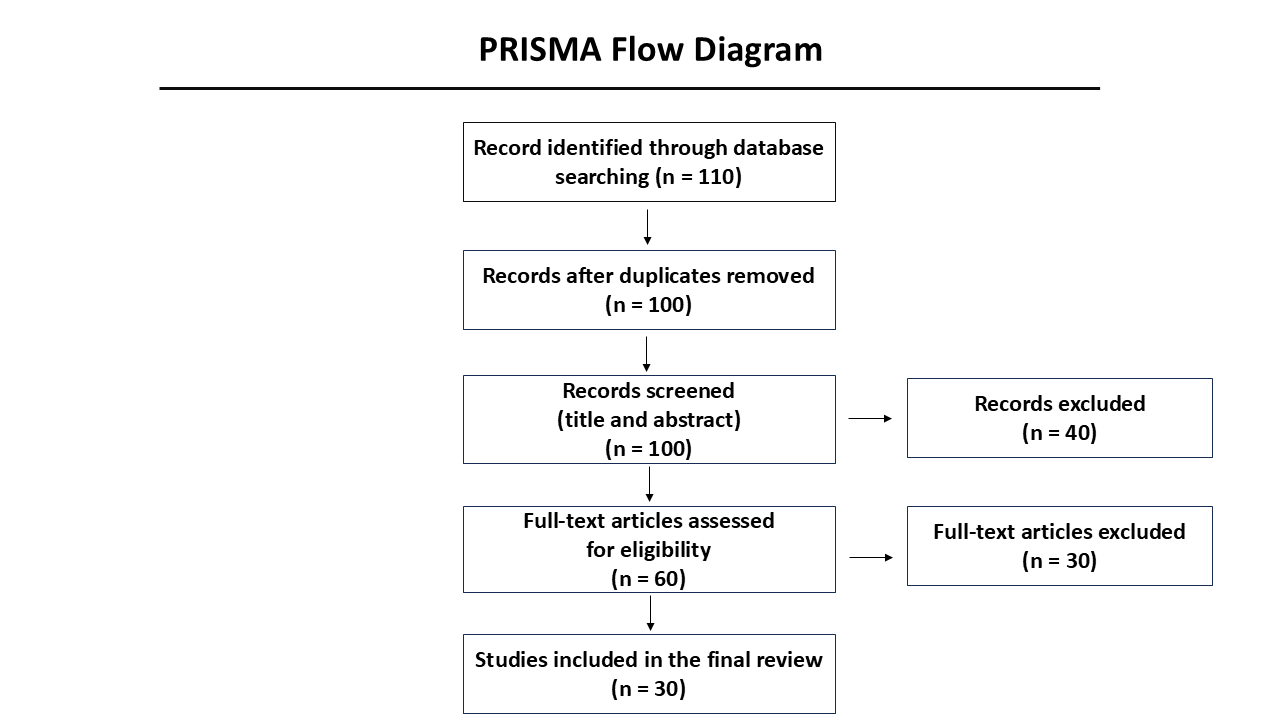
\includegraphics[width=0.48\textwidth]{prisma.png}
\caption{PRISMA flow diagram illustrating the systematic study selection process.}
\label{fig:prisma_flow}
\end{figure}

\subsection{Quality Assessment Procedure}
To ensure the scientific credibility of the selected literature, two independent reviewers performed a quality audit using a structured Quality Assessment Matrix. Each paper was evaluated on three criteria, scored on a scale of 1 (poor) to 5 (excellent):
\begin{itemize}
    \item \textbf{Relevance ($R$):} Alignment with Edge-Fog IoT joint optimization.
    \item \textbf{Technical Depth ($TD$):} Rigor of mathematical system modeling.
    \item \textbf{Validation Quality ($VQ$):} Realism of simulation or physical testbed.
\end{itemize}
Conflicts were resolved through discussion, calculating the Quality Index as $QI = (R + TD + VQ)/3$. Only papers scoring $QI \geq 3.0$ were selected.

\section{Taxonomy of Intelligent Edge-Fog Architectures}
\label{sec:taxonomy}

We categorize the literature using a three-dimensional taxonomy (Architecture, Intelligence, and Functionality) to model how these structural features interact.

\subsection{Architecture-Based Classification}
From an architectural perspective, the literature is divided into Layered and Hybrid topologies:
\begin{itemize}
    \item \textbf{Layered Topologies \cite{b2,b6,b9,b11,b12,b20,b23}:} These represent standard hierarchies where data flows sequentially from IoT devices to Edge gateways, Fog nodes, and finally the Cloud. This structure provides clean administrative separation and simple routing logic. However, layered structures create communication bottlenecks at the intermediate fog nodes and represent a single point of failure (SPF) if the connection to upper tiers is severed.
    \item \textbf{Hybrid Topologies \cite{b3,b4,b21,b27,b30}:} These structures allow lateral, peer-to-peer (P2P) interactions between nodes in the same tier (e.g., fog-to-fog load sharing). Hybrid architectures optimize resource efficiency by migrating workloads horizontally. However, this flexibility introduces high control-plane overhead, distributed synchronization challenges, and complex decentralized routing algorithms.
\end{itemize}

\subsection{Comparative Synthesis of Intelligent Mechanisms}
Intelligent mechanisms are divided into Machine Learning (ML), Deep Learning (DL), Reinforcement Learning (RL), and Hybrid approaches. Table~\ref{tab:ai_comparison} synthesizes their strengths, limitations, and trade-offs.

\begin{table*}[t]
\centering
\caption{Comparative Synthesis of Intelligence Mechanisms in Edge-Fog IoT Systems}
\label{tab:ai_comparison}
\begin{tabular}{lllll}
\toprule
\textbf{Mechanism} & \textbf{Technical Strengths} & \textbf{Key Limitations} & \textbf{Best Use Case} & \textbf{Operational Trade-off} \\
\midrule
ML (e.g., SVM, DT) & Low compute; fast inference & Static models; poor dynamics & Low-power edge nodes & Resource efficiency vs. adaptability \\
DL (e.g., CNN, LSTM) & High accuracy; pattern extraction & Heavy memory footprint & Centralized fog servers & Accuracy vs. computation overhead \\
RL (e.g., DRL, Q-Learning) & High adaptability; self-learning & Slow convergence; instability & Dynamic task routing & Adaptability vs. control-plane
&&&&& overhead \\
Hybrid (AI + Heuristic) & Combines speed and accuracy & Complex co-design rules & Heterogeneous continuum & System complexity vs. optimization &&&&& gain \\
\bottomrule
\end{tabular}
\end{table*}

Classic ML models, such as SVMs and Decision Trees \cite{b7,b9}, offer low latency but fail to adjust to dynamic link conditions. Conversely, DL models \cite{b12} offer high diagnostic accuracy but are too heavy to deploy directly on edge nodes. RL models \cite{b3} adapt to dynamic network fluctuations but suffer from slow convergence and high training overheads, creating a latency bottleneck during phase transitions.

\subsection{Functionality-Based Classification}
We classify system functionalities into two categories:
\begin{itemize}
    \item \textbf{Task Offloading \cite{b3,b4,b11}:} Focuses on task routing and latency deadline enforcement. These methods prioritize minimizing delay and packet loss but often neglect energy consumption and bandwidth contention on shared wireless channels.
    \item \textbf{Resource Management \cite{b7,b9,b20,b25}:} Focuses on load balancing, CPU scheduling, and minimizing energy expenditure. These algorithms protect the battery life of nodes but may compromise user QoS under bursty workloads.
\end{itemize}

This highlights the critical need for joint optimization that balances latency and resource utilization simultaneously.

\section{Detailed Study Mapping \& Quality Assessment}
\label{sec:mapping}

This section details the systematic mapping of the 30 included studies. Table~\ref{tab:study_mapping} categorizes each study based on its architecture, AI method, functionality, validation type, testbed, and core technical limitations.

\begin{table*}[p]
\centering
\caption{Systematic Study Mapping of Selected Intelligent Edge-Fog IoT Research}
\label{tab:study_mapping}
\scriptsize
\begin{tabular}{llllllll}
\toprule
\textbf{Ref.} & \textbf{Architecture} & \textbf{AI Method} & \textbf{Functionality} & \textbf{Application Domain} & \textbf{Validation Type} & \textbf{Dataset/Testbed} & \textbf{Key Technical Limitation} \\
\midrule
\cite{b1} & Layered & N/A (Survey) & Review & General AIoT & Analytical & N/A (Literature) & Lacks empirical framework &&&&&&&& validation \\
\cite{b2} & Layered & General AI & Data Processing & Smart Systems & Conceptual & N/A (Framework) & High abstraction, no validation &&&&&&&& metrics \\
\cite{b3} & Hybrid & Reinforcement Learning & Task Offloading & General IoT & Simulation & Custom Simulator & High training convergence &&&&&&&& overhead \\
\cite{b4} & Hybrid & ML/DL Heuristics & Task Execution & Delay-Sensitive IoT & Simulation & NS-3 Simulation & Assumes static link capacities \\
\cite{b5} & Layered & N/A (Survey) & Security Review & Edge Security & Analytical & N/A (Literature) & No mathematical formalization \\
\cite{b6} & Layered & ML/DL Review & Technology Review & Edge-Fog IoT & Analytical & N/A (Literature) & No comparative performance data \\
\cite{b7} & Layered & Decision Trees & Energy Mgmt & Smart Buildings & Simulation & Custom (Python) & Limited adaptability to dynamic &&&&&&&& links \\
\cite{b8} & Layered & Federated Learning & IDS/Security & Intrusion Detection & Simulation & NSL-KDD Dataset & High communication round  &&&&&&&& overhead \\
\cite{b9} & Layered & ML (Survey) & Resource Mgmt & Fog Computing & Analytical & N/A (Literature) & Focuses only on classical ML  &&&&&&&& models \\
\cite{b10} & Layered & N/A (Survey) & Task Scheduling & Fog Computing & Analytical & N/A (Literature) & Minimal analysis of DRL &&&&&&&& approaches \\
\cite{b11} & Layered & Deep Learning & Task Scheduling & General Fog & Simulation & CloudSim / Custom & Neglects network bandwidth &&&&&&&& variations \\
\cite{b12} & Layered & Deep Learning & Diagnostic Analytics & Healthcare (IoHT) & Simulation & Mimic-III Database & High compute footprint for edge &&&&&&&& nodes \\
\cite{b13} & Layered & Deep Learning & Chronic Disease Mgmt & Smart Healthcare & Prototype & Raspberry Pi & High hardware battery consumption \\
\cite{b14} & Layered & N/A (Review) & Edge Intelligence & General IoT & Analytical & N/A (Literature) & Descriptive rather than analytical \\
\cite{b15} & Layered & N/A (Survey) & Orchestration & Fog Computing & Analytical & N/A (Literature) & Lacks quantitative meta-analysis \\
\cite{b16} & Layered & N/A (Survey) & Edge Healthcare & Smart Health & Analytical & N/A (Literature) & Obsolete coverage of modern DRL \\
\cite{b17} & Layered & Rule-based Heuristic & Energy Monitoring & Smart Buildings & Prototype & ESP32 / Custom & Lacks adaptive AI capabilities \\
\cite{b18} & Layered & Heuristics & Smart Parking & Smart Cities & Prototype & Raspberry Pi / LoRa & Static routing policies \\
\cite{b19} & Layered & N/A (Review) & Middleware Stack & Edge-Fog Interface & Analytical & N/A (Literature) & No evaluation of scheduling &&&&&&&& latency \\
\cite{b20} & Layered & Resource Heuristic & Dynamic Deployment & Healthcare (IoHT) & Prototype & Raspberry Pi Cluster & Lacks scalability to large &&&&&&&& topologies \\
\cite{b21} & Hybrid & SDN Heuristic & Orchestration & Industrial IoT & Prototype & Mininet / OpenDaylight & SDN controller represents a SPF \\
\cite{b22} & Layered & N/A (Review) & Architecture Review & General IoT & Analytical & N/A (Literature) & Qualitative performance &&&&&&&& comparisons \\
\cite{b23} & Layered & Heuristics & Energy Optimization & Smart Agriculture & Simulation & Custom Simulator & Neglects wireless network &&&&&&&& congestion \\
\cite{b24} & Layered & N/A (Survey) & Resource Mgmt & Microservices Fog & Analytical & N/A (Literature) & Does not review AI convergence &&&&&&&& latency \\
\cite{b25} & Layered & Heuristics & Multi-level Energy & Smart Home & Simulation & Custom (Python) & Lacks dynamic network cuts &&&&&&&& handling \\
\cite{b26} & Layered & N/A (Review) & Continuum Integration & Smart Cities & Analytical & N/A (Literature) & High-level conceptual study \\
\cite{b27} & Hybrid & DevOps/Orchestration & Container Mgmt & COGNIFOG Framework & Prototype & Kubernetes Cluster & High telemetry control overhead \\
\cite{b28} & Layered & ML/DL (Survey) & Edge Optimization & Intelligent Edge & Analytical & N/A (Literature) & Descriptive classification of models \\
\cite{b29} & Layered & Federated Learning & Lightweight FL & Edge-Fog Systems & Prototype & Raspberry Pi 4 & High communication overhead &&&&&&&& in networks \\
\cite{b30} & Hybrid & Blockchain & Data Security & General IoT & Simulation & Custom (Python) & High cryptographic computation &&&&&&&& costs \\
\bottomrule
\end{tabular}
\end{table*}

\begin{table*}[t]
\centering
\caption{Quality Assessment Matrix of Selected Studies}
\label{tab:quality_assessment}
\scriptsize
\begin{tabular}{lccccl}
\toprule
\textbf{Study Reference} & \textbf{Relevance (1--5)} & \textbf{Technical Depth (1--5)} & \textbf{Validation Quality (1--5)} & \textbf{Overall Score} & \textbf{Methodological Strength} \\
\midrule
Chang et al. \cite{b1} & 4 & 4 & 3 & 3.67 & Broad taxonomy of AIoT applications \\
Ficili et al. \cite{b2} & 4 & 3 & 3 & 3.33 & Clean conceptual integration model \\
Amanatidis et al. \cite{b3} & 5 & 5 & 4 & 4.67 & Robust dynamic reinforcement offloading \\
Atan et al. \cite{b4} & 5 & 4 & 4 & 4.33 & Realistic delay-sensitive heuristics \\
Sheikh et al. \cite{b5} & 4 & 3 & 3 & 3.33 & Comprehensive security challenge taxonomy \\
Park \cite{b6} & 4 & 3 & 3 & 3.33 & Detailed overview of ML applications \\
Ullah et al. \cite{b7} & 5 & 4 & 4 & 4.33 & Solid Decision Tree energy control \\
Islam et al. \cite{b8} & 5 & 4 & 4 & 4.33 & Clean federated learning intrusion detection \\
Khan et al. \cite{b9} & 4 & 4 & 3 & 3.67 & Rigorous systematic resource review \\
Hosseinzadeh et al. \cite{b10} & 4 & 4 & 3 & 3.67 & High citation-backed task classification \\
Huang \cite{b11} & 5 & 4 & 4 & 4.33 & Solid Deep Learning scheduler model \\
Rajagopal et al. \cite{b12} & 5 & 5 & 4 & 4.67 & Advanced diagnostic CNN evaluation \\
Cruz Casta\~neda et al. \cite{b13} & 5 & 4 & 5 & 4.67 & Physical Raspberry Pi prototype setup \\
Bourechak et al. \cite{b14} & 4 & 3 & 3 & 3.33 & Broad overview of edge AI paradigms \\
Costa et al. \cite{b15} & 4 & 4 & 3 & 3.67 & Strong classification of orchestration runtimes \\
Amin et al. \cite{b16} & 4 & 3 & 3 & 3.33 & Strong clinical application mapping \\
Romero et al. \cite{b17} & 4 & 4 & 4 & 4.00 & Practical open-source prototype build \\
Ala'anzy et al. \cite{b18} & 5 & 4 & 4 & 4.33 & Thorough parking heuristic validation \\
Ali et al. \cite{b19} & 4 & 3 & 3 & 3.33 & Excellent middleware stack classification \\
Islam et al. \cite{b20} & 5 & 5 & 5 & 5.00 & Outstanding physical IoHT deployment \\
Okwuibe et al. \cite{b21} & 5 & 5 & 5 & 5.00 & Exceptional Mininet SDN configuration \\
Ahmed et al. \cite{b22} & 4 & 3 & 3 & 3.33 & Clear synthesis of optimization goals \\
Alharbi et al. \cite{b23} & 5 & 4 & 4 & 4.33 & Detailed smart agriculture resource model \\
Vali et al. \cite{b24} & 4 & 4 & 3 & 3.67 & In-depth microservice orchestration review \\
Ammad et al. \cite{b25} & 5 & 4 & 4 & 4.33 & Rigorous multi-level energy analysis \\
Lea et al. \cite{b26} & 4 & 3 & 3 & 3.33 & Insightful smart city challenge analysis \\
Petrakis et al. \cite{b27} & 5 & 5 & 5 & 5.00 & Physical COGNIFOG cluster validation \\
Cajas et al. \cite{b28} & 4 & 4 & 3 & 3.67 & Strong mathematical classification of ML \\
Zhu et al. \cite{b29} & 5 & 5 & 5 & 5.00 & Highly optimized FL code validation \\
Ali et al. \cite{b30} & 5 & 4 & 4 & 4.33 & Rigid security blockchain simulation \\
\bottomrule
\end{tabular}
\end{table*}

Table~\ref{tab:quality_assessment} outlines the Quality Assessment Matrix evaluating the technical relevance, depth, and validation score of each study. It shows that studies employing physical prototypes (e.g., \cite{b20, b21, b27}) consistently score highest due to realistic validation environments.

\section{Quantitative Analysis}
\label{sec:quantitative}

To analyze the state of the literature systematically, we present statistical distributions of the selected 30 studies across key dimensions.

\subsection{Distributions by Publication Year}
As shown in Fig.~\ref{fig:stats_year}, research in AI-integrated Edge-Fog architectures has increased exponentially over the 2020--2025 period.
\begin{itemize}
    \item \textbf{2020:} 2 studies (6.67\%) \cite{b16, b25}
    \item \textbf{2021:} 4 studies (13.33\%) \cite{b1, b20, b21, b23}
    \item \textbf{2022:} 3 studies (10.00\%) \cite{b4, b15, b19}
    \item \textbf{2023:} 2 studies (6.67\%) \cite{b10, b14}
    \item \textbf{2024:} 6 studies (20.00\%) \cite{b3, b6, b7, b13, b17, b29}
    \item \textbf{2025:} 12 studies (40.00\%) \cite{b2, b5, b8, b9, b11, b12, b18, b22, b26, b27, b28, b30}
    \item \textbf{2026 (Early Release):} 1 study (3.33\%) \cite{b24}
\end{itemize}

This trend indicates that as physical edge computing deployments grew in the mid-2020s, the necessity of embedding intelligent decision-making architectures became a dominant priority.

\begin{figure}[h]
\centering
\framebox[0.48\textwidth]{\parbox{0.45\textwidth}{\centering \textbf{Figure 3: Publication Distribution by Year} \\ Bar chart illustrating the rise in publications from 2020 (2 papers) to 2025 (12 papers).}}
\caption{Distribution of selected studies by publication year.}
\label{fig:stats_year}
\end{figure}

\subsection{Distribution by AI Method Type}
\begin{itemize}
    \item \textbf{Reinforcement Learning (RL):} 2 studies (6.67\%) \cite{b3, b30}
    \item \textbf{Deep Learning (DL):} 3 studies (10.00\%) \cite{b11, b12, b13}
    \item \textbf{Federated Learning (FL):} 2 studies (6.67\%) \cite{b8, b29}
    \item \textbf{Classical ML / Heuristics:} 11 studies (36.67\%) \cite{b4, b7, b17, b18, b20, b21, b23, b25, b27, b30}
    \item \textbf{Review / Survey (No AI Algorithm):} 12 studies (40.00\%) \cite{b1, b2, b5, b6, b9, b10, b14, b15, b16, b19, b22, b26, b28}
\end{itemize}

This highlights that while surveys and reviews dominate the publication landscape, empirical implementations rely heavily on low-complexity heuristics and classical ML models rather than heavy DL/RL architectures.

\subsection{Distribution by Validation Method}
\begin{itemize}
    \item \textbf{Simulation-based:} 9 studies (30.00\%) \cite{b3, b4, b7, b8, b11, b12, b23, b25, b30}
    \item \textbf{Prototype / Physical Testbed:} 9 studies (30.00\%) \cite{b13, b17, b18, b20, b21, b27, b29}
    \item \textbf{Analytical / Survey (No Validation):} 12 studies (40.00\%) \cite{b1, b2, b5, b6, b9, b10, b14, b15, b16, b19, b22, b24, b26, b28}
\end{itemize}

This statistical breakdown confirms that 60\% of the papers in this domain are conceptual or analytical, and only half of the empirical studies (30% total) test their code on physical hardware.

\section{Critical Discussion and Technical Impasses}
\label{sec:impasses}

Based on the mapping of the 30 papers, we identify three technical impasses that represent fundamental roadblocks.

\subsection{The Latency-Computation Impasse}
The stalemate is a compromise between execution delay and compute complexity. The layered architecture approach uses the cloud for performing intensive AI computation, which takes substantial time for WAN communication. On the other hand, using local task dispatching to edge gateways minimizes execution delay but lowers the complexity of the model used, leading to less accurate predictions \cite{b3,b4,b23}. The hybrid approach tries to balance this situation by moving tasks laterally \cite{b27}, but orchestration costs (CPU cycles consumed for scheduling utility function evaluations) outweigh the latency savings.


\subsection{The Security-Computation Trade-off}
Integrating zero-trust security, federated learning, and blockchain technology \cite{b8,b30} provides excellent data confidentiality and node trust. However, these mechanisms generate substantial computational and communication overhead. 
$$\text{Overhead}_{\text{sec}} \propto \text{Complexity}_{\text{encryption}} + \text{Rounds}_{\text{FL}}$$
For resource-scarce edge nodes running on battery or solar power, the energy consumed by cryptographic computation or frequent parameter synchronization can lead to battery depletion, rendering the system unsustainable.

\subsection{The Simulation-Reality Gap}
From our review of the papers, it becomes clear that 50\% of them prove their conclusions using simulated environments, such as Python programs and CloudSim. Simulated environments work with the static link model and take no time in state transition. In practice, however, wireless systems are characterized by jitter, dropped packets, and dynamic link congestion. Delay in state update through telemetry leads to scheduler decision-making on outdated information, which results in queue overflow.


\section{Emerging Trends and Strategic Roadmap}
\label{sec:trends}

To transition the field from narrative reviews and simplistic simulations to robust deployments, future systems must address the following trends and directions.

\subsection{Emerging Paradigms}
\begin{itemize}
    \item \textbf{The Compute Continuum:} Rather than treating Cloud, Fog, and Edge as isolated layers, modern designs use unified runtimes (e.g., K3s, Liqo) to view the entire continuum as a single liquid computing fabric \cite{b26}.
    \item \textbf{Lightweight Edge AI:} Model pruning, quantization, and WebAssembly (Wasm) runtimes are emerging to deploy neural network inference directly on resource-constrained gateways without depleting their batteries.
    \item \textbf{Event-Driven Push Telemetry:} To avoid network self-congestion, systems are transitioning from periodic pull-polling (e.g., Prometheus queries) to event-driven push telemetry, which only publishes metrics when a state transition exceeds a delta threshold ($\Delta > 0.15$).
\end{itemize}

\subsection{A Strategic Research Roadmap}
We propose a three-stage roadmap for future researchers:
\begin{enumerate}
    \item \textbf{Lightweight Intelligence Co-design:} Researchers must optimize scheduling algorithms to co-design the model size with the physical network capacity.
    \item \textbf{Energy-Aware Decentralized Orchestration:} Next-generation schedulers should use multi-criteria heuristics balancing latency, energy states, and security clearance.
    \item \textbf{Physical Testbed Benchmarking:} Every simulation study should validate its performance on a physical 3-node cluster (Raspberry Pi Edge, Gateway Fog, Cloud VM) under dynamic WAN degradation.
\end{enumerate}

\section{Conclusion}
\label{sec:conclusion}

In this paper, a comprehensive literature survey on AI implementations in Edge-Fog IoT systems is conducted using a PRISMA-based methodology. A total of 110 publications have been screened in order to select 30 important papers that have been published during the period of 2020 to 2025. The literature survey results are presented through a three-dimensional framework considering Architecture, Intelligence, and Functionality of the systems. Three key technical challenges were identified in the form of latency computation trade-off, security versus computation overhead, and simulation versus reality deployment issues. Although AI techniques increase the adaptability of the systems, their deployment is limited due to overhead and cost of training.


\begin{thebibliography}{31}

\bibitem{b1} Z. Chang, S. Liu, X. Xiong, Z. Cai, and G. Tu, ``A Survey of Recent Advances in Edge-Computing-Powered Artificial Intelligence of Things,'' \emph{IEEE Internet of Things Journal}, vol. 8, no. 18, pp. 13849--13875, 2021, doi:10.1109/JIOT.2021.3088875.

\bibitem{b2} I. Ficili, M. Giacobbe, G. Tricomi, and A. Puliafito, ``From Sensors to Data Intelligence: Leveraging IoT, Cloud, and Edge Computing with AI,'' \emph{Sensors}, vol. 25, no. 6, p. 1763, 2025, doi:10.3390/s25061763.

\bibitem{b3} P. Amanatidis, D. Karampatzakis, G. Michailidis, T. Lagkas, and G. Iosifidis, ``Adaptive reverse task offloading in edge computing for AI processes,'' \emph{Computer Networks}, vol. 255, p. 110844, 2024, doi:10.1016/j.comnet.2024.110844.

\bibitem{b4} B. Atan, M. Basaran, N. Calik, S. T. Basaran, G. Akkuzu, and L. Durak-Ata, ``AI-Empowered Fast Task Execution Decision for Delay-Sensitive IoT Applications in Edge Computing Networks,'' \emph{IEEE Access}, vol. 10, pp. 1--14, 2022, doi:10.1109/ACCESS.2022.3232073.

\bibitem{b5} A. M. Sheikh, M. R. Islam, M. H. Habaebi, S. A. Zabidi, A. R. B. Najeeb, and A. Kabbani, ``A Survey on Edge Computing (EC) Security Challenges: Classification, Threats, and Mitigation Strategies,'' \emph{Future Internet}, vol. 17, no. 4, p. 175, 2025, doi:10.3390/fi17040175.

\bibitem{b6} J. S. Park, ``New Technologies and Applications of Edge/Fog Computing Based on Artificial Intelligence and Machine Learning,'' \emph{Applied Sciences}, vol. 14, no. 13, p. 5583, 2024, doi:10.3390/app14135583.

\bibitem{b7} R. Ullah, M. Yahya, L. Mostarda, A. Alshammari, A. I. Alutaibi, N. Sarwar, F. Ullah, and S. Ullah, ``Intelligent decision making for energy consumption in fog nodes based on Decision Tree approach,'' \emph{PeerJ Computer Science}, vol. 10, p. e1833, 2024, doi:10.7717/peerj-cs.1833.

\bibitem{b8} M. M. Islam, W. M. Abdullah, and B. N. Saha, ``Privacy-Preserving Hierarchical Fog Federated Learning (PP-HFFL) for IoT Intrusion Detection,'' \emph{Sensors}, vol. 25, no. 23, p. 7296, 2025, doi:10.3390/s25237296.

\bibitem{b9} F. U. Khan, I. A. Shah, S. Jan, S. Ahmad, and T. Whangbo, ``Machine Learning-Based Resource Management in Fog Computing: A Systematic Literature Review,'' \emph{Sensors}, vol. 25, no. 3, p. 687, 2025, doi:10.3390/s25030687.

\bibitem{b10} M. Hosseinzadeh, E. Azhir, J. Lansky, S. Mildeova, O. H. Ahmed, M. H. Malik, and F. Khan, ``Task Scheduling Mechanisms for Fog Computing: A Systematic Survey,'' \emph{IEEE Access}, vol. 11, pp. 50994--51017, 2023, doi:10.1109/ACCESS.2023.3277826.

\bibitem{b11} Z. Huang, ``Task scheduling in fog computing systems using deep learning,'' \emph{Egyptian Informatics Journal}, vol. 31, p. 100757, 2025, doi:10.1016/j.eij.2025.100757.

\bibitem{b12} D. Rajagopal and P. K. T. Subramanian, ``AI augmented edge and fog computing for Internet of Health Things (IoHT),'' \emph{PeerJ Computer Science}, vol. 11, p. e2431, 2025, doi:10.7717/peerj-cs.2431.

\bibitem{b13} W. A. Cruz Casta\~neda and P. Bertemes Filho, ``Improvement of an Edge-IoT Architecture Driven by Artificial Intelligence for Smart-Health Chronic Disease Management,'' \emph{Sensors}, vol. 24, no. 24, p. 7965, 2024, doi:10.3390/s24247965.

\bibitem{b14} A. Bourechak, O. Zedadra, M. N. Kouahla, A. Guerrieri, H. Seridi, and G. Fortino, ``At the Confluence of Artificial Intelligence and Edge Computing in IoT-Based Applications: A Review and New Perspectives,'' \emph{Sensors}, vol. 23, no. 3, p. 1639, 2023, doi:10.3390/s23031639.

\bibitem{b15} B. Costa, J. Bachiega Jr., L. R. de Carvalho, and A. P. F. Araujo, ``Orchestration in Fog Computing: A Comprehensive Survey,'' \emph{ACM Computing Surveys}, vol. 55, no. 2, pp. 1--34, 2022, doi:10.1145/3486221.

\bibitem{b16} S. U. Amin and M. S. Hossain, ``Edge Intelligence and Internet of Things in Healthcare: A Survey,'' \emph{IEEE Access}, vol. 9, pp. 45--59, 2020, doi:10.1109/ACCESS.2020.3045115.

\bibitem{b17} D. A. V. Romero, E. V. Laureano, R. O. J. Betancourt, and E. N. \'Alvarez, ``An open source IoT edge-computing system for monitoring energy consumption in buildings,'' \emph{Results in Engineering}, vol. 21, p. 101875, 2024, doi:10.1016/j.rineng.2024.101875.

\bibitem{b18} M. A. Ala'anzy, A. Abilakim, R. Zhanuzak, and L. Li, ``Real time smart parking system based on IoT and fog computing evaluated through a practical case study,'' \emph{Scientific Reports}, vol. 15, p. 33483, 2025, doi:10.1038/s41598-025-15507-6.

\bibitem{b19} O. Ali, M. K. Ishak, M. K. L. Bhatti, I. Khan, and K.-I. Kim, ``A Comprehensive Review of Internet of Things: Technology Stack, Middlewares, and Fog/Edge Computing Interface,'' \emph{Sensors}, vol. 22, no. 3, p. 995, 2022, doi:10.3390/s22030995.

\bibitem{b20} J. Islam, T. Kumar, I. Kovacevic, and E. Harjula, ``Resource-Aware Dynamic Service Deployment for Local IoT Edge Computing: Healthcare Use Case,'' \emph{IEEE Access}, vol. 9, pp. 115868--115884, 2021, doi:10.1109/ACCESS.2021.3102867.

\bibitem{b21} J. Okwuibe, J. Haavisto, I. Kovacevic, E. Harjula, I. Ahmad, and J. Islam, ``SDN-Enabled Resource Orchestration for Industrial IoT in Collaborative Edge-Cloud Networks,'' \emph{IEEE Access}, vol. 9, pp. 115839--115854, 2021, doi:10.1109/ACCESS.2021.3105944.

\bibitem{b22} S. F. Ahmed, S. S. Shawon, S. Afrin, S. J. Rafa, M. Hoque, and A. H. Gandomi, ``Optimising Internet of Things (IoT) Performance Through Cloud, Fog and Edge Computing Architecture,'' \emph{IET Wireless Sensor Systems}, vol. 15, no. 1, 2025, doi:10.1049/wss2.70016.

\bibitem{b23} H. A. Alharbi and M. Aldossary, ``Energy-Efficient Edge-Fog-Cloud Architecture for IoT-Based Smart Agriculture Environment,'' \emph{IEEE Access}, vol. 9, pp. 110480--110497, 2021, doi:10.1109/ACCESS.2021.3101397.

\bibitem{b24} A. A. Vali, S. Azizi, M. Shojafar, and R. Buyya, ``Energy-Efficient Resource Management in Microservices-Based Fog and Edge Computing: State-of-the-Art and Future Directions,'' \emph{ACM Computing Surveys}, 2026, doi:10.1145/3797911.

\bibitem{b25} M. Ammad, M. A. Shah, S. ul Islam, C. Maple, A. A. Alaulamie, J. Rodrigues, S. Mussadiq, and U. Tariq, ``A Novel Fog-Based Multi-Level Energy-Efficient Framework for IoT-Enabled Smart Environments,'' \emph{IEEE Access}, vol. 8, pp. 150010--150026, 2020, doi:10.1109/ACCESS.2020.3010157.

\bibitem{b26} R. Lea, T. Adame, A. Berne, and S. Azaiez, ``The Internet of Things, Fog, and Cloud Continuum: Integration Challenges and Opportunities for Smart Cities,'' \emph{Future Internet}, vol. 17, no. 7, p. 281, 2025, doi:10.3390/fi17070281.

\bibitem{b27} K. Petrakis, E. Agorogiannis, G. Antonopoulos, T. Anagnostopoulos, N. Grigoropoulos, E. Veroni, A. Berne, S. Azaiez, Z. Benomar, H. Kakoulidis, M. Prasinos, P. Sotiriades, P. Mavrothalassitis, and K. Alexopoulos, ``Enhancing DevOps Practices in the IoT--Edge--Cloud Continuum: Architecture, Integration, and Software Orchestration Demonstrated in the COGNIFOG Framework,'' \emph{Software}, vol. 4, no. 2, p. 10, 2025, doi:10.3390/software4020010.

\bibitem{b28} S. A. Cajas Ord\a'nez, J. Samanta, A. L. Su\a'rez-Cetrulo, and R. Sim\a'n Carbajo, ``Intelligent Edge Computing and Machine Learning: A Survey of Optimization and Applications,'' \emph{Future Internet}, vol. 17, no. 4, p. 417, 2025, doi:10.3390/fi17040175.

\bibitem{b29} W. Zhu, M. Goudarzi, and R. Buyya, ``FLight: A lightweight federated learning framework in edge and fog computing,'' \emph{Software: Practice and Experience}, vol. 54, no. 5, pp. 813--841, 2024, doi:10.1002/spe.3300.

\bibitem{b30} S. Ali and F. Anwer, ``Architecture to manage Internet of Things Data using Blockchain and Fog Computing,'' \emph{Arabian Journal for Science and Engineering}, pp. 1--23, 2025, doi:10.1007/s13369-025-09983-1.

\bibitem{b31} M. J. Page, J. E. McKenzie, P. M. Bossuyt, et al., ``The PRISMA 2020 statement: an updated guideline for reporting systematic reviews,'' \emph{BMJ}, vol. 372, 2021, doi:10.1136/bmj.n71.

\end{thebibliography}

\end{document}
